In diesem Kapitel wird die Durchf\"uhrung des Versuches beschrieben.


% **************************************************************************** %
\subsection{Versuchsanordnung}
\label{sec:durchf:subsec:anordn}
% **************************************************************************** %

%\begin{figure}[th!]
%    \centering
%    \includegraphics[width=.5\textwidth]{images/versuchsanordnung.jpeg}
%    \caption{Die Versuchsanordnung}
%\end{figure}
%\begin{figure}[th!]
%    \centering
%    \includegraphics[width=.5\textwidth]{images/blockschaltbild.jpeg}
%    \caption{Die Versuchsanordnung}
%\end{figure}

% Picture and Tools

% **************************************************************************** %
\subsection{Versuchsablauf}
\label{sec:durchf:subsec:ablauf}
% **************************************************************************** %


% ---------------------------------------------------------------------------- %
\subsubsection{Hohlzylinder}
% ---------------------------------------------------------------------------- %

\begin{figure}[th!]
    \centering
    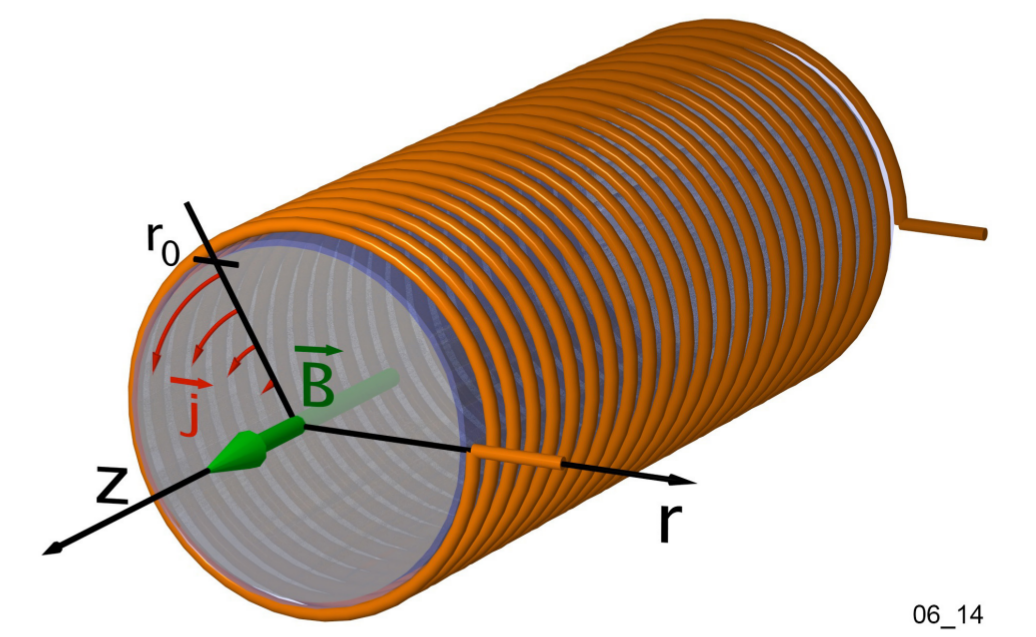
\includegraphics[width=.5\textwidth]{images/spule-vollzylinder.png}
    \caption{Spule mit Vollzylinder \emph{Quelle:} Skript zum Versuch}
\end{figure}


% ---------------------------------------------------------------------------- %
\subsubsection{Vollzylinder}
% ---------------------------------------------------------------------------- %

\begin{figure}[th!]
    \centering
    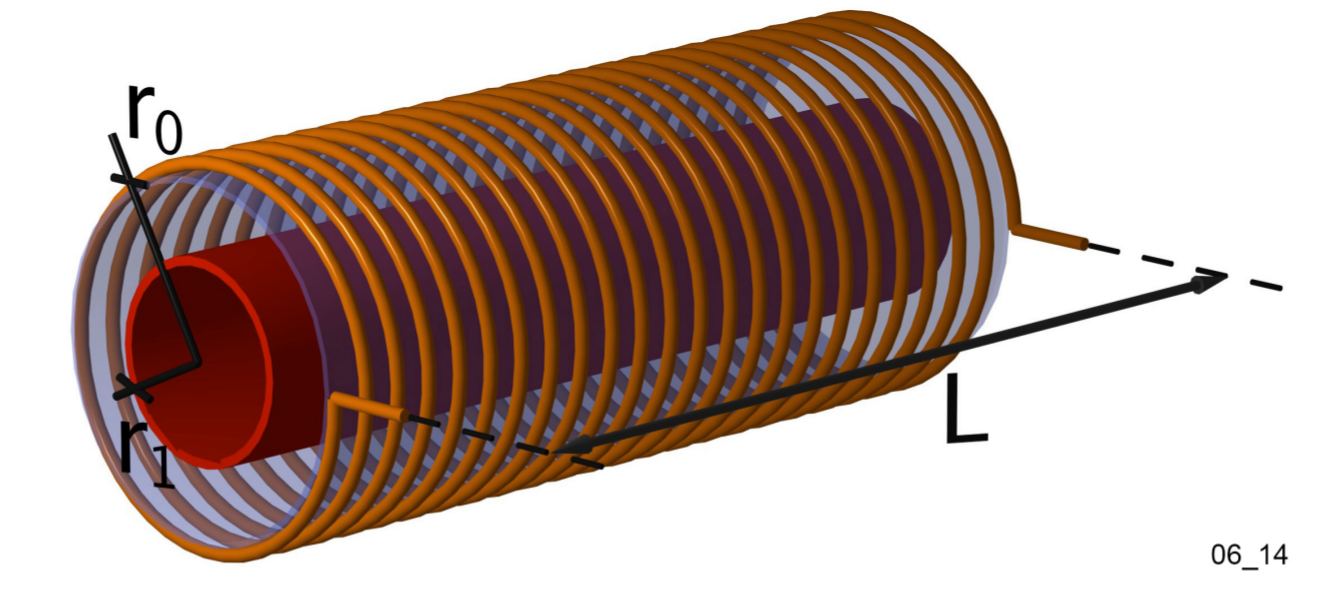
\includegraphics[width=.5\textwidth]{images/spule-hohlzylinder.png}
    \caption{Spule mit Hohlzylinder \emph{Quelle:} Skript zum Versuch}
\end{figure}
